% !TEX root = ../my-thesis.tex
%
\chapter{Appendix}
\label{sec:appendix}

\section{Drone data processing methodology}
\label{sec:drone_method}

\begin{figure}
	\begin{center}
		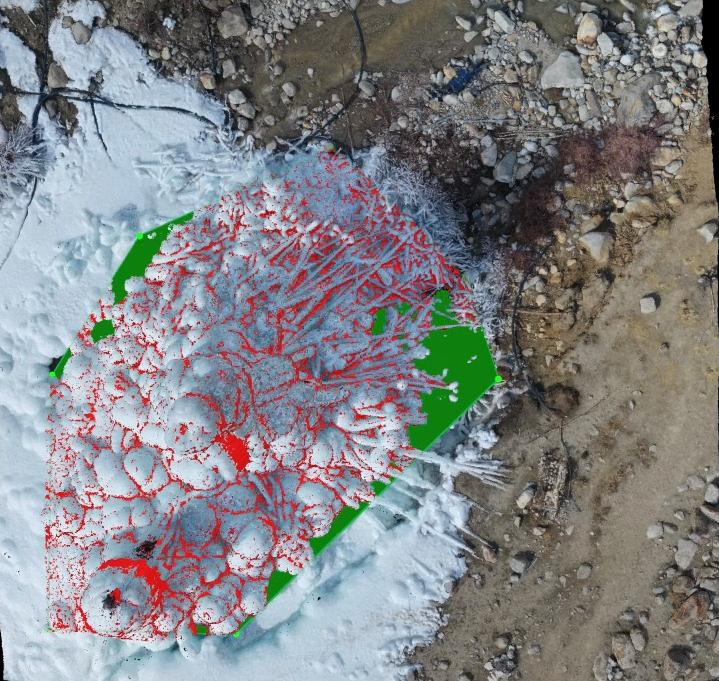
\includegraphics[width=12 cm]{figs/pix4d.jpg}
	\end{center}
	\caption{Digital elevation map of Indian AIR constructed from the drone survey on March 3, 2021. The green
		area represents the area bounded by the marked perimeter and the red area represents gaps in the point cloud
    that were filled to compute the associated volume.
	}
	\label{fig:DEM}
\end{figure}

The drone flew automatically along a predefined flight course and took photographs at a certain time interval. The
position and altitude of the drone at the exposure stations, which were obtained by the built-in integrated
Position and Orientation System (POS, composed of a global positioning system and inertial measurement units),
were recorded in JPEG pictures. In this study, we adopted a three-step workflow as implemented in the
commercial software package Pix4Dmapper version 4.6.4 (\cite{Pix4D}). A short summary of this workflow is
described below:

(1) Initial processing: This process generates a sparse point cloud with the structure-from motion algorithm
(\cite{Turner_2012}). First, it searches for and matches key points in the photos that have certain overlapping
areas using a feature matching algorithm (e.g., the scale-invariant feature transform (SIFT) algorithm, which can
detect key points in photos with different views and illumination conditions; \cite{Lowe_2004}). Second, the
approximate locations and orientations of the camera at each exposure station are reconstructed with the internal
parameters (focal length, coordinates of the principal point of the photograph), and external parameters (i.e. POS
data). A sparse point cloud is created.

(2) Point cloud densification: In this step, the multi-view stereo technique is applied to achieve a higher point
cloud density than in the previous step (\cite{Furukawa_2010}; \cite{Molg_2017}). Thus, the spatial resolution of
the products can be increased, and an irregular network for the next step can be created (\cite{Kung_2011}).

(3) AIR delineation: Ice radius, area and volume are the three final products. Perimeter was manually marked
on the point cloud by identifying the AIR boundary (see Fig. \ref{fig:DEM}). For the Indian location, we identified identical rock features
near the ice boundary to mark as vertices of this perimeter. For the Swiss AIR, no such feature was available due
to snowfall, so instead the perimeter was marked by identifying the ice and snow boundary.

There is temporal and spatial uncertainty associated with this process. Weather conditions influence the quality
of each drone survey variably. Moreover, since ice/snow surfaces do not have many identifiable features, few
feature points can be detected and matched in the vicinity of the AIR. Thus, we attach a high uncertainty of
$\pm 10 \%$ for all the AIR observations to accommodate for this.

\section{Ladakh AIRs dataset}
\label{sec:appendix:sec1}

\Blindtext[1][1]

\begin{table}[h]
	\begin{tabularx}{\textwidth}{X | X | X}
		%\hline
		Alpha		& Beta			& Gamma			\\ \hline
		0			& 1				& 2				\\ \hline
		3			& 4				& 5				\\ %\hline
	\end{tabularx}
	\label{tab:table1}
	\caption{This is a caption text.}
\end{table}

\section{Appendix Section 2}
\label{sec:appendix:sec2}

\Blindtext[1][1]

\begin{table}[h]
	\begin{tabularx}{\textwidth}{X | X | X}
		%\hline
		Alpha		& Beta			& Gamma			\\ \hline
		0			& 1				& 2				\\ \hline
		3			& 4				& 5				\\ %\hline
	\end{tabularx}
	\label{tab:table2}
	\caption{This is a caption text.}
\end{table}

\Blindtext[1][2]
